\documentclass[11pt]{article}
\usepackage[margin=1in]{geometry}
\usepackage{amsmath,amssymb}
\usepackage{booktabs}
\usepackage{graphicx}
\usepackage[american]{circuitikz}
\usetikzlibrary{positioning,arrows.meta,calc,fit,backgrounds}
\usepackage[colorlinks=true,linkcolor=blue,citecolor=blue,urlcolor=blue]{hyperref}
\usepackage{caption}
\captionsetup{font=small,labelfont=bf}

\newcommand{\eps}{\varepsilon}
\ctikzset{transistors/scale=0.7}

\title{Learning Entirely in Circuit Dynamics:\\
Sign-Faithful Error Transport Enables Deep Analog Predictive Coding}
\author{Thomas D.\ Ahle\thanks{Draft v0.2. All reported numbers are transistor-level Cadence Spectre transient-simulation results; no behavioral elements appear in any training or inference path.}}
\date{June 2026}

\begin{document}
\maketitle

\begin{abstract}
We present an analog CMOS learning system in which \textbf{both inference and learning are physical circuit dynamics}: weights are charge on capacitors, neurons and synapses are small transistor cells, prediction errors are voltages on explicit circuit nodes, and weight updates are currents produced by local four-quadrant multiplier cells. An external controller only cycles training data and supplies bias and clock voltages---it performs no computation. The system implements continuous predictive coding as two simultaneous gradient flows: neural states settle fast ($\dot h \propto -\partial E/\partial h$) while weights charge slowly ($\dot W \propto -\eta\,\partial E/\partial W$). We report four main results, all validated by simulating the \emph{entire training process} as a single transistor-level SPICE transient. \textbf{(1)} A \emph{soft $\beta$-nudge output clamp}---replacing the conventional hard label clamp with a weak resistive pull, as required by equilibrium-propagation theory in the small-nudge limit---is decisive for learning quality, raising the spirals benchmark from 1/4 to 4/4 seeds above 95\%; with two initialization fixes the system exceeds 95\% on every seed of three nonlinear 2D tasks. \textbf{(2)} The system scales to 64-input handwritten digits: 89.0\% on 4 classes (backprop ideal on the identical sparse topology: 91--94\%) and 58.7\% on 10 classes, and we quantify an accuracy-per-component trade-off in which a fixed-random-feature variant keeps 74\% accuracy with 42\% fewer transistors and 80\% fewer capacitors. \textbf{(3)} Deep credit assignment through chained analog transposes fails by \emph{error-alignment decay}; we introduce \textbf{sign-faithful error transport}---one comparator per neuron regenerating error \emph{signs} to full swing at each layer---which lifts a depth-4 network from 55\% to 84\% at $\sim$14 extra transistors per hidden neuron and makes curriculum schedules unnecessary. \textbf{(4)} As a generality probe, the hardware also runs predictive coding's native unsupervised mode (input prediction): an in-circuit masked autoencoder learns above chance with no labels, though its features do not beat random projections downstream, and we report that control. We further characterize an $N{+}1$-transistor competition cell computing an exactly normalized, sparsemax-sharp distribution, and we measure the system's chief vulnerability: static transistor mismatch of $\sigma=2\,$mV degrades the depth-4 result from 0.84 to 0.46, a first-class negative result that sets the agenda for offset-canceling cell design. We distill the campaign into measured design laws for physical learning machines.
\end{abstract}

\section{Introduction}

Backpropagation on digital hardware dominates machine learning, but it is strikingly unlike learning in physical and biological systems: it requires storing and transporting exact weight matrices, global synchronization, and high-precision arithmetic. Analog electronics promises orders-of-magnitude efficiency gains, yet nearly all analog AI hardware accelerates only \emph{inference}; training remains exiled to a digital host. The brain hints at a third option: a physical dynamical system whose ordinary time-evolution \emph{is} both inference and learning.

This paper asks how far that idea can be pushed with ordinary CMOS transistors, under deliberately brain-like constraints: neurons of roughly 4-bit effective precision, fan-in and fan-out of at most $\sim$4--10, no weight transport, purely local plasticity, and a controller that does nothing but present data. Concretely, we build a small library of transistor cells (Section~\ref{sec:cells})---synapses, neurons, error subtractors, and update multipliers---wire them into sparse multi-layer networks, and let the circuit's own differential equations carry out predictive-coding inference \emph{and} weight updates. Every quantity in the algorithm is a voltage or a current somewhere in the netlist, and an entire training run (thousands of example presentations) is one continuous transient simulation.

Why insist on simulating training at transistor level, rather than abstracting the circuit into equations? Because the abstractions fail in instructive ways. During this campaign we built a device-equation surrogate that matched the circuit's per-step behavior to 10--30\% and still mispredicted long-horizon training outcomes; the real circuit exploits effects---load compression, common-mode-shaped errors---that the abstraction discards (Section~\ref{sec:limits}). The mechanism-level findings of Section~\ref{sec:laws}, each established by direct circuit measurement, are in our view the paper's most durable contribution.

\subsection{Related work}
\label{sec:related}

\paragraph{Energy-based training of analog networks.} Equilibrium propagation (EP) \cite{scellier2017} showed that energy-based models can estimate loss gradients from two settled network states. Kendall et al.~\cite{kendall2020} brought EP to analog hardware in simulation: a single-hidden-layer (100-unit) network whose weights are ideal programmable \emph{conductances} (memristors) and whose nonlinearities are diodes, trained to 96.6\% on MNIST in Spectre. Our system differs in kind: synapses, neurons, error cells, and---critically---the weight-update computation itself are transistor circuits; learning is one continuous transient (no two-phase state storage, no externally computed updates); and we address depth, which crossbar EP leaves open. Follow-ups include memristor-crossbar EP \cite{oh2023}, circuit-compatibility theory for EP via adjoint/reciprocity methods \cite{lirmm2025}, and comparative studies of energy-based analog learning \cite{scellier2023comp}.

\paragraph{Physical learning machines.} Dillavou et al.~\cite{dillavou2022} demonstrated decentralized contrastive ``coupled learning'' in real electronics---the closest work in spirit. Their networks are \emph{linear} resistor networks with digitally stepped variable resistors (128 levels) and twin-network comparison circuitry, solving small tasks; we are nonlinear, deep, continuous-weight, and single-network, but simulation-only where they have hardware. Wright et al.~\cite{wright2022} train physical systems with digitally computed physics-aware backprop; Momeni et al.~\cite{momeni2023} remove backprop but still compute local losses digitally. Concurrent work pursues fully-analog training on other substrates: photonics via perturbative gradient measurement \cite{photonic2025} and a spintronic-CMOS spiking neuron \cite{spintronic2025}---different learning principles from our continuous predictive-coding dynamics.

\paragraph{Analog learning chips.} On-chip learning in analog VLSI has a long heritage: 1990s self-learning chips implemented perceptron or backprop rules in weak-inversion translinear circuits with capacitor or floating-gate weights \cite{cauwenberghs1996}, typically small and with parts of the loop off-chip. Modern in-memory computing trains memristor arrays in situ with \emph{digital} optimizers \cite{yao2020}; BrainScaleS-2 pairs analog neurons with an embedded digital plasticity processor \cite{pehle2022}. Relative to all of these, our claim is narrow and specific: at transistor level, the complete learning loop---error computation, credit assignment through depth, and the multiply that drives each weight---runs as continuous, simultaneous circuit dynamics with no digital or behavioral element in the loop.

\section{Background for the general reader}
\label{sec:background}

\subsection{Five circuit facts}
\label{sec:primer}

Readers comfortable with transistors may skip ahead. Five facts make everything below intelligible.

\begin{enumerate}
\item \textbf{A MOS transistor is a voltage-controlled current valve.} Raising the gate voltage of an NMOS transistor lets more current flow from drain to source. Over a useful range the relationship is smooth and saturating---a free nonlinearity.
\item \textbf{Wires add for free.} By Kirchhoff's current law, currents flowing into the same node sum. An analog ``dot product'' is therefore just many synapse cells dumping current onto one wire.
\item \textbf{Differential signaling.} Every signal $u$ in this paper is carried by a \emph{pair} of wires as a difference, $u \equiv V(u_p)-V(u_n)$, straddling a common-mode (average) level around mid-supply. Differences cancel shared disturbances and represent negative numbers naturally.
\item \textbf{A capacitor integrates current: } $C\,\dot V = I$. A capacitor holding charge is a memory; a small current pushed onto it is a \emph{learning-rate-scaled update}. Our weights are capacitor voltages.
\item \textbf{SPICE} (we use Cadence Spectre) numerically integrates the coupled nonlinear ODEs of all transistor currents and capacitor charges---a brute-force, physics-faithful simulation. If training works in such a transient, the dynamics, not an idealization, did the work.
\end{enumerate}

All cells use a two-type LEVEL-1 process (NMOS $V_{T}=0.2$\,V, PMOS $V_{T}=-0.2$\,V, $\textsc{kp}=120/40\,\mu$A/V$^2$, $\lambda=0.02$, $V_{DD}=1$\,V). Device sizes are W/L as marked in the figures; signal common modes sit near $0.45$--$0.65$\,V.

\subsection{Predictive coding as a pair of gradient flows}
\label{sec:pc}

Predictive coding (PC) \cite{rao1999,whittington2017} structures a network around \emph{predictions} and \emph{errors}. Layer $\ell$ holds value nodes $x_\ell$; the layer below it produces a prediction $m_\ell = f(W_\ell\, a_{\ell-1})$ of those values (where $a_{\ell-1}=f(x_{\ell-1})$ are activations); the mismatch is an explicit error signal
\[
\eps_\ell \;=\; x_\ell - m_\ell ,
\]
and the whole network descends the energy
\[
E \;=\; \tfrac12 \sum_\ell \lVert x_\ell - m_\ell \rVert^2 .
\]
Two gradient flows run \emph{simultaneously} at separated time scales:
\begin{align}
\text{fast (inference):}\quad & \dot x_\ell \;\propto\; -\frac{\partial E}{\partial x_\ell} \;=\; -\eps_\ell + W_{\ell+1}^{\!\top}\!\big(f'\circ\eps_{\ell+1}\big), \label{eq:fast}\\[2pt]
\text{slow (learning):}\quad & \dot W_\ell \;\propto\; -\eta\,\frac{\partial E}{\partial W_\ell} \;=\; \eta\;\eps_\ell\, a_{\ell-1}^{\!\top}. \label{eq:slow}
\end{align}
Equation~\eqref{eq:fast} says a value node is pulled toward its own prediction and simultaneously nudged by errors it causes upstream; Eq.~\eqref{eq:slow} is a purely \emph{local} product---this synapse's error times this synapse's input---which is what makes a hardware implementation plausible. Supervision enters by pulling the output-layer values toward a target $y$; with everything clamped appropriately and small nudging, the weight flow follows the supervised loss gradient (the equilibrium-propagation result \cite{scellier2017}). In our circuit, Eq.~\eqref{eq:fast} is enforced by synaptic currents on value nodes ($\sim$8\,ns settling), and Eq.~\eqref{eq:slow} by multiplier cells charging weight capacitors over milliseconds, while the controller presents one example per 400\,ns slot. The time-scale separation is provided by capacitor sizing, not by sequencing.

\section{The cell library}
\label{sec:cells}

\subsection{Synapse: degenerated Gilbert multiplier (\texttt{gsyn}, 7T)}

A synapse must compute (signed input)\,$\times$\,(signed weight) as an output \emph{current}. The classic circuit is the Gilbert cell (Fig.~\ref{fig:gsyn}): a bottom differential pair steers the tail current according to the weight voltage $w$, and an upper cross-coupled quad steers each branch according to the input $u$; the cross-coupling makes the output differential current proportional to the \emph{product} of the two tanh-compressed inputs:
\[
I_{\text{out}} \;\approx\; -\,G \cdot \tanh(2.25\,u)\cdot \tanh(k_w\,w), \qquad G \approx 0.105 \text{ (measured)} .
\]
Note the inversion (a wiring-level fact our netlists must respect). The six $12\,\mathrm{k}\Omega$ \emph{source-degeneration} resistors linearize each pair (measured fit quality $R^2$: $0.92 \to 0.99$); without them, nonlinear benchmark tasks fail. Weights arrive as the differential capacitor voltage $(w_p, w_n)$.

\begin{figure}[t]
\centering
\begin{circuitikz}[scale=0.82, transform shape]
% tail
\draw (5.0,0) node[nmos](Mt){} ;
\draw (Mt.S) -- ++(0,-0.3) node[ground]{};
\draw (Mt.G) -- ++(-0.7,0) node[left,font=\scriptsize]{$v_{b}$};
\draw (Mt.D) -- ++(0,0.35);
\draw (2.3,0.95) -- (7.7,0.95);
\node[circ] at (5.0,0.95){}; \node[right=2pt,font=\scriptsize] at (5.05,1.15) {$n_t$};
% weight pair
\draw (2.3,2.5) node[nmos](M5){} (7.7,2.5) node[nmos](M6){};
\draw (M5.G) -- ++(-0.6,0) node[left,font=\scriptsize]{$w_p$};
\draw (M6.G) -- ++(-0.6,0) node[left,font=\scriptsize]{$w_n$};
\draw (M5.S) to[R] (2.3,0.95);
\draw (M6.S) to[R] (7.7,0.95);
% branch rails na nb
\draw (M5.D) -- ++(0,0.4); \draw (M6.D) -- ++(0,0.4);
\draw (0.8,3.7) -- (3.8,3.7); \node[circ] at (2.3,3.7){}; \node[font=\scriptsize] at (2.05,3.95) {$n_a$};
\draw (6.2,3.7) -- (9.2,3.7); \node[circ] at (7.7,3.7){}; \node[font=\scriptsize] at (7.45,3.95) {$n_b$};
% upper quad
\draw (0.8,5.3) node[nmos](M1){} (3.8,5.3) node[nmos](M2){} (6.2,5.3) node[nmos](M3){} (9.2,5.3) node[nmos](M4){};
\draw (M1.S) to[R] (0.8,3.7);
\draw (M2.S) to[R] (3.8,3.7);
\draw (M3.S) to[R] (6.2,3.7);
\draw (M4.S) to[R] (9.2,3.7);
\draw (M1.G) -- ++(-0.6,0) node[left,font=\scriptsize]{$u_p$};
\draw (M2.G) -- ++(-0.6,0) node[left,font=\scriptsize]{$u_n$};
\draw (M3.G) -- ++(-0.6,0) node[left,font=\scriptsize]{$u_p$};
\draw (M4.G) -- ++(-0.6,0) node[left,font=\scriptsize]{$u_n$};
% outputs: M2+M3 -> outn (short low rail); M1+M4 -> outp (long high rail, no crossings)
\draw (M2.D) -- ++(0,0.55) -- ++(0.5,0) coordinate(onl);
\draw (M3.D) -- ++(0,0.55) -- (onl) node[circ]{};
\node[font=\scriptsize] at (5.3,6.75) {$i_{\text{out},n}$};
\draw (M1.D) -- ++(0,1.5) -- ++(8.4,0) coordinate(opr) node[circ]{} node[right=2pt,font=\scriptsize]{$i_{\text{out},p}$};
\draw (M4.D) -- ++(0,1.5);
\end{circuitikz}
\caption{\textbf{Synapse \texttt{gsyn}} (7 NMOS + 6 source-degeneration resistors, all $12\,\mathrm{k}\Omega$; tail 400/100, all others 200/100\,$\mu$m). The weight pair (gates $w_p,w_n$) splits the tail current between branch rails $n_a, n_b$; the cross-coupled input quad (gates $u_p,u_n$) steers each branch to the two output wires ($u_p$ pulls $i_{\text{out},p}$ from the $n_a$ side but $i_{\text{out},n}$ from the $n_b$ side---that crossing is the multiply). Result: $I_{\text{out}} \approx -G\tanh(2.25u)\tanh(k_w w)$, $G{\approx}0.105$. Output is a \emph{current}, so many synapses sum on a wire for free (fact 2). Mind the sign inversion.}
\label{fig:gsyn}
\end{figure}

\subsection{Neuron and common-mode load (\texttt{dneuron} + \texttt{cmld}, 3T+2T)}

The neuron (Fig.~\ref{fig:dneuron}, left) is a differential pair with a tail current sink: its output is a saturating function of the input voltage, measured as
\[
a \;=\; 0.537\,\tanh(15.7\,u)\,,
\]
i.e., a sharp tanh---effectively a 4-bit activation, in line with our design philosophy. Its load is the \texttt{cmld} cell (Fig.~\ref{fig:dneuron}, right): two resistors sense the output pair's average (common mode) at node $cm_x$, which drives two PMOS gates in feedback, pinning the average while presenting high resistance to the \emph{difference}. Without this cell, common-mode levels drift layer by layer and the cascade dies; with it, every layer hands the next a signal centered where the next cell wants it.

\begin{figure}[t]
\centering
\begin{circuitikz}[scale=0.9, transform shape]
% dneuron
\draw (1.0,1.6) node[nmos](N1){} (3.4,1.6) node[nmos](N2){};
\draw (2.2,-0.2) node[nmos](Nt){};
\draw (N1.S) -- ++(0,-0.35) -| (Nt.D);
\draw (N2.S) -- ++(0,-0.35) -| (Nt.D);
\draw (Nt.S) -- ++(0,-0.3) node[ground]{};
\draw (Nt.G) -- ++(-0.6,0) node[left,font=\scriptsize]{$v_{b}$};
\draw (N1.G) -- ++(-0.5,0) node[left,font=\scriptsize]{$u_p$};
\draw (N2.G) -- ++(-0.5,0) node[left,font=\scriptsize]{$u_n$};
\draw (N1.D) -- ++(0,0.55) node[circ]{} node[left,font=\scriptsize]{$a_n$};
\draw (N2.D) -- ++(0,0.55) node[circ]{} node[right,font=\scriptsize]{$a_p$};
\node at (2.2,-1.85) [font=\scriptsize] {\texttt{dneuron}: $a = 0.537\tanh(15.7\,u)$};
% cmld
\begin{scope}[xshift=7.2cm]
\draw (0.3,2.8) node[pmos](P1){} (4.5,2.8) node[pmos,xscale=-1](P2){};
\draw (P1.S) -- ++(0,0.4) node[vcc]{\scriptsize$V_{DD}$};
\draw (P2.S) -- ++(0,0.4) node[vcc]{\scriptsize$V_{DD}$};
\draw (P1.D) -- ++(0,-0.9) node[circ]{} coordinate(p) node[right=2pt,font=\scriptsize]{$p$};
\draw (P2.D) -- ++(0,-0.9) node[circ]{} coordinate(n) node[left=2pt,font=\scriptsize]{$n$};
\draw (p) -- ++(0,-0.55) coordinate(pl);
\draw (n) -- ++(0,-0.55) coordinate(nl);
\draw (pl) to[R,l_=\scriptsize$R_{cs}$] ($(pl)!0.5!(nl)$) coordinate(cmx);
\draw (cmx) to[R,l_=\scriptsize$R_{cs}$] (nl);
\node[circ] at (cmx){};
\draw (cmx) -- ++(0,-0.45) coordinate(cmlow) node[below,font=\scriptsize]{$cm_x$};
\draw (cmlow) -- ++(-3.3,0) |- (P1.G);
\draw (cmlow) -- ++(3.3,0) |- (P2.G);
\node at (2.4,-1.2) [font=\scriptsize] {\texttt{cmld}: pins $(V_p{+}V_n)/2$, high impedance to $V_p{-}V_n$};
\end{scope}
\end{circuitikz}
\caption{\textbf{Left: neuron \texttt{dneuron}} (differential pair + tail). \textbf{Right: common-mode-feedback load \texttt{cmld}}. The two $R_{cs}$ average the outputs; that average drives both PMOS gates, so any common-mode rise is fed back and cancelled, while differential signals see only the large PMOS output resistance. Every \texttt{dneuron} output and every value node carries one.}
\label{fig:dneuron}
\end{figure}

\subsection{Error cell (\texttt{esub}, 5T)}

PC needs $\eps = x - m$ as a real signal. The \texttt{esub} cell (Fig.~\ref{fig:esub}) is a four-input shared-tail stage: transistors gated by $x_p$ and $m_n$ pull down the $\eps_n$ side, and those gated by $x_n$ and $m_p$ pull down the $\eps_p$ side, so with resistor loads the differential output is
\[
\eps \;\propto\; (x_p - x_n) - (m_p - m_n) \;=\; x - m, \qquad \text{gain } 2.5 \text{ at matched common modes.}
\]
A measured subtlety that matters in practice: when its two input pairs sit at \emph{different} common-mode levels (e.g.\ a label clamp at 0.50\,V vs.\ a prediction at 0.65\,V), the transfer becomes $\eps \approx 1.66\,(0.66\,x - m)$---the lower-CM input is attenuated. Real analog error signals are CM-skewed versions of $x-m$ (design law \#2).

\begin{figure}[t]
\centering
\begin{circuitikz}[scale=0.9, transform shape]
\draw (0.5,2.0) node[nmos](E1){} (3.2,2.0) node[nmos](E2){} (6.2,2.0) node[nmos](E3){} (8.9,2.0) node[nmos](E4){};
\draw (4.7,0.1) node[nmos](Et){};
\foreach \m in {E1,E2,E3,E4} \draw (\m.S) -- ++(0,-0.3) -| (Et.D);
\draw (Et.S) -- ++(0,-0.3) node[ground]{};
\draw (Et.G) -- ++(-0.6,0) node[left,font=\scriptsize]{$v_b$};
\draw (E1.G) -- ++(-0.45,0) node[left,font=\scriptsize]{$x_n$};
\draw (E2.G) -- ++(-0.45,0) node[left,font=\scriptsize]{$m_p$};
\draw (E3.G) -- ++(-0.45,0) node[left,font=\scriptsize]{$x_p$};
\draw (E4.G) -- ++(-0.45,0) node[left,font=\scriptsize]{$m_n$};
% loads: E1,E2 -> ep ; E3,E4 -> en
\draw (E1.D) -- ++(0,0.5) -- ++(1.0,0) coordinate(ep) node[circ]{};
\draw (E2.D) -- ++(0,0.5) -- (ep);
\draw (E3.D) -- ++(0,0.5) -- ++(1.0,0) coordinate(en) node[circ]{};
\draw (E4.D) -- ++(0,0.5) -- (en);
\node[below right=1pt and 0pt of ep,font=\scriptsize]{$\eps_p$};
\node[below right=1pt and 0pt of en,font=\scriptsize]{$\eps_n$};
\draw (ep) to[R,l=\scriptsize$50\mathrm{k}$] ++(0,1.6) node[vcc]{\scriptsize$V_{DD}$};
\draw (en) to[R,l=\scriptsize$50\mathrm{k}$] ++(0,1.6) node[vcc]{\scriptsize$V_{DD}$};
\end{circuitikz}
\caption{\textbf{Error cell \texttt{esub}}: a four-input shared-tail differential stage computing $\eps \propto x - m$ (gain 2.5 at matched common modes). The cross-assignment of gates to output sides implements the subtraction; the measured CM-imbalance law $\eps \approx 1.66(0.66x - m)$ applies when input common modes differ.}
\label{fig:esub}
\end{figure}

\subsection{Update cell (\texttt{gprod}, 15T) and the weight capacitor}

Equation~\eqref{eq:slow} requires a four-quadrant product $\eps \cdot a$ delivered as a current onto the weight capacitors. The \texttt{gprod} cell (Fig.~\ref{fig:gprod}) is a degenerated Gilbert core (like \texttt{gsyn}) whose differential output current is then \emph{rectified into a push--pull pair}: diode-connected PMOS devices sense the two branch currents; mirror transistors push the $i_p$ image onto $w_p$ and, via an NMOS mirror, pull the $i_n$ image off it (and symmetrically for $w_n$). The net charging current is
\[
C\,\frac{d}{dt}(w_p - w_n) \;\propto\; \eps \cdot a, \qquad \text{full scale } \pm 8.5\,\mu\text{A (measured)} .
\]
Weights are differential 300\,pF capacitor pairs. The cell is measurably \emph{non-separable}: for small $|\eps|$ and $|a|$ the product is sub-bilinear---a built-in soft deadzone that, in practice, filters update noise. A leak resistor ($R_{WL}=2\,\mathrm{G}\Omega$) to the weight common mode bounds drift on the slowest time scale.

\begin{figure}[t]
\centering
\begin{circuitikz}[scale=0.8, transform shape]
% ---- left: Gilbert core, same layout as gsyn (Fig 1), inputs eps and a ----
\draw (3.4,0) node[nmos](Gt){};
\draw (Gt.S) -- ++(0,-0.3) node[ground]{};
\draw (Gt.G) -- ++(-0.7,0) node[left,font=\scriptsize]{$g_{bl}$};
\draw (Gt.D) -- ++(0,0.3);
\draw (1.6,0.85) -- (5.2,0.85);
\draw (1.6,2.3) node[nmos](G5){} (5.2,2.3) node[nmos](G6){};
\draw (G5.G) -- ++(-0.55,0) node[left,font=\scriptsize]{$a_p$};
\draw (G6.G) -- ++(-0.55,0) node[left,font=\scriptsize]{$a_n$};
\draw (G5.S) to[R] (1.6,0.85);
\draw (G6.S) to[R] (5.2,0.85);
\draw (G5.D) -- ++(0,0.35); \draw (G6.D) -- ++(0,0.35);
\draw (0.5,3.45) -- (2.7,3.45);
\draw (4.1,3.45) -- (6.3,3.45);
\draw (0.5,5.0) node[nmos](G1){} (2.7,5.0) node[nmos](G2){} (4.1,5.0) node[nmos](G3){} (6.3,5.0) node[nmos](G4){};
\draw (G1.S) to[R] (0.5,3.45); \draw (G2.S) to[R] (2.7,3.45);
\draw (G3.S) to[R] (4.1,3.45); \draw (G4.S) to[R] (6.3,3.45);
\draw (G1.G) -- ++(-0.5,0) node[left,font=\scriptsize]{$\eps_p$};
\draw (G2.G) -- ++(-0.5,0) node[left,font=\scriptsize]{$\eps_n$};
\draw (G3.G) -- ++(-0.5,0) node[left,font=\scriptsize]{$\eps_p$};
\draw (G4.G) -- ++(-0.5,0) node[left,font=\scriptsize]{$\eps_n$};
\draw (G2.D) -- ++(0,0.5) -- ++(0.35,0) coordinate(gon);
\draw (G3.D) -- ++(0,0.5) -- (gon) node[circ]{};
\node[font=\scriptsize] at (3.75,6.3) {$i_{on}$};
\draw (G1.D) -- ++(0,1.3) -- ++(5.8,0) node[circ]{} node[right=2pt,font=\scriptsize]{$i_{op}$};
\draw (G4.D) -- ++(0,1.3);
% ---- right: push-pull output stage onto w_p ----
\begin{scope}[xshift=8.9cm,yshift=0.6cm]
\draw (0.0,4.6) node[pmos,xscale=-1](Pl){};
\draw (Pl.S) -- ++(0,0.3) node[vcc]{\scriptsize$V_{DD}$};
\draw (Pl.D) -- ++(0,-0.6) coordinate(iopn) node[circ]{} node[below,font=\scriptsize]{$i_{op}$ in};
\draw (Pl.G) -| (iopn);
\draw (2.8,4.6) node[pmos](Pu){};
\draw (Pu.S) -- ++(0,0.3) node[vcc]{\scriptsize$V_{DD}$};
\draw (Pu.G) -- ++(-1.0,0) |- ($(Pl.G)+(0.25,0)$);
\draw (Pu.D) -- ++(0,-1.6) coordinate(wp) node[circ]{} node[right=3pt,font=\scriptsize]{$w_p$};
\draw (wp) to[C,l_=\scriptsize$300\,\mathrm{p}$] ++(-2.0,0) node[ground]{};
\draw (wp) -- ++(0,-1.1) coordinate(wpd);
\draw (6.2,4.6) node[pmos](Pr){};
\draw (Pr.S) -- ++(0,0.3) node[vcc]{\scriptsize$V_{DD}$};
\draw (Pr.G) -- ++(-0.8,0) node[left,font=\scriptsize]{$i_{on}$ in};
\draw (Pr.D) -- ++(0,-1.2) coordinate(nrn) node[circ]{} node[left=3pt,font=\scriptsize]{$n_{rn}$};
\draw (6.2,1.0) node[nmos,xscale=-1](Nd){};
\draw (Nd.D) -- (nrn);
\draw (Nd.G) -- ++(0.35,0) coordinate(ndg) (ndg) |- (nrn);
\draw (Nd.S) -- ++(0,-0.3) node[ground]{};
\draw (2.8,1.0) node[nmos,xscale=-1](Npd){};
\draw (Npd.D) -- (wpd);
\draw (Npd.G) -- ++(0.35,0) -- ++(0,-0.85) -| (ndg);
\draw (Npd.S) -- ++(0,-0.3) node[ground]{};
\node at (3.4,-1.6) [font=\scriptsize,align=center] {push--pull: $I(w_p)\propto i_{op}-i_{on}$\\ ($w_n$ stage = mirror image, 4 more devices)};
\end{scope}
\end{circuitikz}
\caption{\textbf{Update cell \texttt{gprod}} (15T). Left: a degenerated Gilbert core (same topology as Fig.~\ref{fig:gsyn}, inputs $\eps$ and $a$) computes the four-quadrant product as a differential current pair $(i_{op},i_{on})$. Right: a diode-connected PMOS senses $i_{op}$ and a mirror pushes its image onto the weight capacitor, while the $i_{on}$ image is folded through an NMOS mirror that pulls charge off the same node. Net: $C\,\dot w \propto \eps\, a$ ($\pm8.5\,\mu$A full scale)---Eq.~\eqref{eq:slow} as physics.}
\label{fig:gprod}
\end{figure}

\subsection{One layer assembled}

Figure~\ref{fig:system} shows the dataflow of one hidden layer. Forward \texttt{gsyn} cells (one per connection, fan-in $\le 4$) sum prediction currents on $m$ nodes; \texttt{esub} computes $\eps = x - m$; a backward path injects upstream error into $x$ (closing the fast flow, Eq.~\eqref{eq:fast}); \texttt{gprod} cells integrate $\eps \cdot a$ onto their weight capacitors (the slow flow, Eq.~\eqref{eq:slow}); the same capacitor voltage drives the forward \texttt{gsyn}. The supervised clamp is a resistor: the controller's label voltage pulls each output value node through $R_{\text{clamp}} = 120\,\mathrm{k}\Omega$, realizing the soft $\beta$-nudge of Section~\ref{sec:softclamp} with $\beta \approx 0.17$.

\begin{figure}[t]
\centering
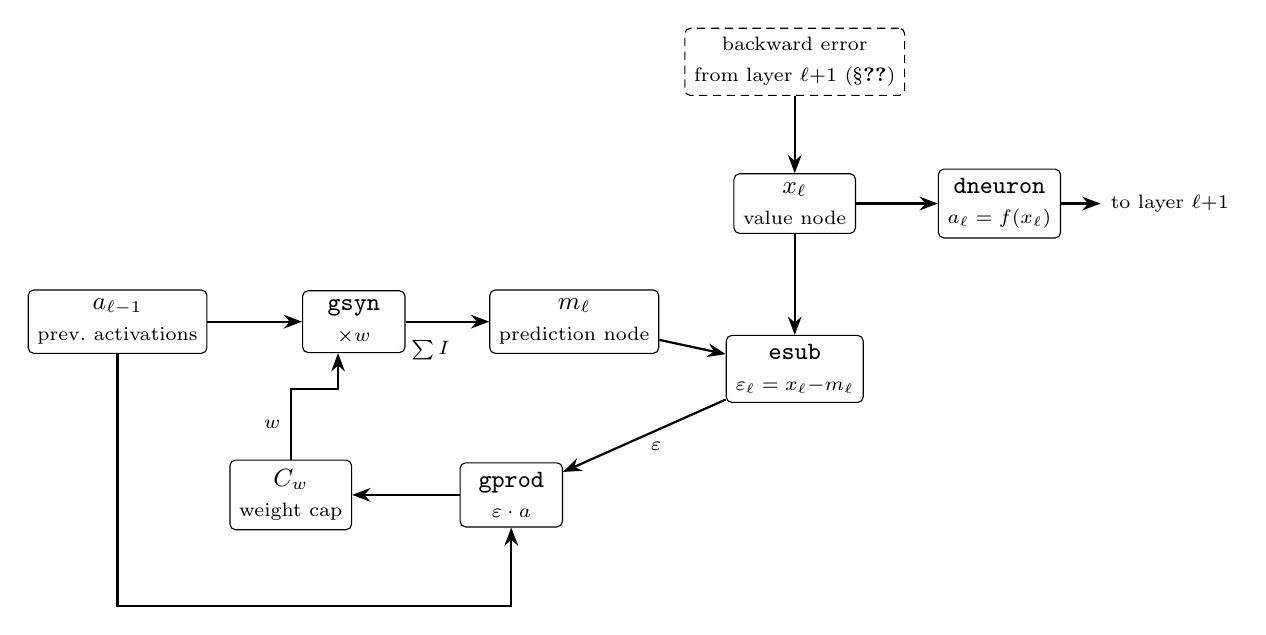
\begin{tikzpicture}[font=\small,
  box/.style={draw, rounded corners=2pt, minimum height=7mm, minimum width=13mm, align=center},
  sig/.style={-{Stealth}, thick}]
\node[box] (apre) at (0,0) {$a_{\ell-1}$\\ \scriptsize prev.\ activations};
\node[box] (gsyn) at (3.0,0) {\texttt{gsyn}\\ \scriptsize $\times w$};
\node[box] (m) at (5.8,0) {$m_\ell$\\ \scriptsize prediction node};
\node[box] (x) at (8.6,1.5) {$x_\ell$\\ \scriptsize value node};
\node[box] (esub) at (8.6,-0.6) {\texttt{esub}\\ \scriptsize $\eps_\ell = x_\ell{-}m_\ell$};
\node[box] (gprod) at (5.0,-2.2) {\texttt{gprod}\\ \scriptsize $\eps\cdot a$};
\node[box] (cap) at (2.2,-2.2) {$C_w$\\ \scriptsize weight cap};
\node[box] (dn) at (11.2,1.5) {\texttt{dneuron}\\ \scriptsize $a_\ell = f(x_\ell)$};
\node[box,densely dashed] (bk) at (8.6,3.3) {\scriptsize backward error\\ \scriptsize from layer $\ell{+}1$ (\S\ref{sec:bksign})};
\draw[sig] (apre) -- (gsyn);
\draw[sig] (gsyn) -- node[below=3pt,pos=0.3]{\scriptsize $\sum I$} (m);
\draw[sig] (m) -- (esub);
\draw[sig] (x) -- (esub);
\draw[sig] (bk) -- (x);
\draw[sig] (esub) -- node[below right=-2pt]{\scriptsize $\eps$} (gprod);
\draw[sig] (apre.south) -- ++(0,-3.2) -| (gprod.south);
\draw[sig] (gprod) -- (cap);
\draw[sig] (cap.north) -- ++(0,0.9) node[midway,left]{\scriptsize $w$} -| ($(gsyn.south)+(-0.2,0)$);
\draw[sig] (x) -- (dn);
\draw[sig] (dn.east) -- ++(0.5,0) node[right]{\scriptsize to layer $\ell{+}1$};
\end{tikzpicture}
\caption{\textbf{One layer of the learning fabric.} All arrows are wires; all boxes are the transistor cells of Figs.~\ref{fig:gsyn}--\ref{fig:gprod}. The loop $C_w \to \texttt{gsyn} \to m \to \texttt{esub} \to \texttt{gprod} \to C_w$ \emph{is} the learning algorithm; nothing outside the schematic computes.}
\label{fig:system}
\end{figure}

\section{Learning dynamics results}

\subsection{The soft $\beta$-nudge clamp}
\label{sec:softclamp}

The textbook way to supervise a PC/EP network is to \emph{clamp} output values to the label with a voltage source---infinitely strong supervision. EP theory \cite{scellier2017} requires the opposite limit: the loss term $\frac{\beta}{2}\lVert y - x_L\rVert^2$ must be \emph{weak} ($\beta$ small) for the weight flow to follow the true gradient. The circuit translation is one resistor: pull the output node toward the label voltage through $R_{\text{clamp}}$, giving an effective $\beta \approx R_{\text{node}}/R_{\text{clamp}} \approx 0.17$.

On the spirals benchmark (deep-narrow net $[2,4,4,4,4,4]$, fan-in 4), the hard clamp yields $0.963/0.912/0.950/0.944$ over four data seeds; the soft clamp yields $\mathbf{0.969/-/0.969/0.956}$, lifting both marginal seeds decisively past $0.95$, reproducibly at two $\beta$ values. With two further initialization findings---structured inits must be explicitly randomized (a deterministic init had silently pinned several ``unsolvable'' seeds), and initial capacitor charge is a legitimate free variable---the system achieves $>\!95\%$ on \textbf{every seed of all three} nonlinear 2D tasks: rings $1.000$ (all seeds), spirals $0.969/0.956/0.969/0.956$, circles $8/8$ seeds (including $0.963$ and $0.988$ on the two formerly locked seeds).

\subsection{Scaling and component economy}

On scikit-learn $8{\times}8$ digits (z-scored, first $C$ classes), with sparse random connectivity (hidden fan-in 4):

\begin{table}[h]
\centering\small
\begin{tabular}{lrrrr}
\toprule
Configuration & FETs & Caps & Update cells & Test acc \\
\midrule
Full plastic, 64--16--16--4 & $\sim$5{,}293 & 360 & 144 & \textbf{0.890} \\
Backprop ideal (same topology, Adam) & --- & --- & --- & 0.91--0.94 \\
Fixed-random hidden, plastic readout & $\sim$3{,}053 & \textbf{72} & 32 & 0.740 \\
10-class, 64--48 random hidden, fan-in-10 readout & $\sim$5{,}507 & 180 & 80 & 0.587 \\
\bottomrule
\end{tabular}
\caption{Scale and component economy (chance is $0.25$ for $C{=}4$, $0.10$ for $C{=}10$).}
\label{tab:scale}
\end{table}

The in-circuit learner sits within $\sim$3 points of the backprop ideal at this scale. Two sizing laws emerged: readout fan-in should be $\approx C$, and the readout must cover $\gtrsim 20\%$ of the feature pool (48 features beat 96 at fan-in 10: $0.587$ vs $0.433$).

\subsection{Depth and sign-faithful error transport}
\label{sec:bksign}

Deep sparse pyramids (64--32--16--8--4, fan-in 4) plateau at $0.55$ under joint training, far below the depth-2 reference ($0.890$). By elimination (hotter hidden learning rates, per-layer backward gain, direct feedback alignment, longer schedules, reshaped curricula---all $\le 0.69$), the failure is \emph{error-alignment decay through chained analog transposes}: each analog stage multiplies the error by a distorted gain, and after several stages the error \emph{direction} is wrong, not just its size.

The repair follows the paper's design philosophy: analog magnitudes degrade per stage; \emph{signs}, if regenerated, do not. Per hidden neuron we add (Fig.~\ref{fig:bksign}): a collector wire summing the backward synapse currents; a \texttt{dneuron} used as a \emph{comparator} (gain ${\approx}16$, saturating) that regenerates the collected error to full swing; and a fixed-negative-unity \texttt{gsyn} injecting the result into the value node. Cost: ${\sim}14$ transistors per hidden neuron, no capacitors.

\begin{figure}[h]
\centering
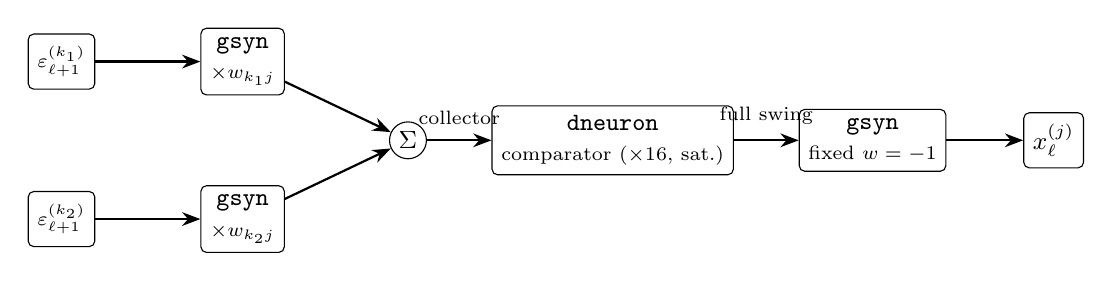
\begin{tikzpicture}[font=\small,
  box/.style={draw, rounded corners=2pt, minimum height=7mm, align=center},
  sig/.style={-{Stealth}, thick}]
\node[box] (e1) at (0,1.0) {\scriptsize $\eps_{\ell+1}^{(k_1)}$};
\node[box] (e2) at (0,-1.0) {\scriptsize $\eps_{\ell+1}^{(k_2)}$};
\node[box] (s1) at (2.3,1.0) {\texttt{gsyn}\\ \scriptsize $\times w_{k_1 j}$};
\node[box] (s2) at (2.3,-1.0) {\texttt{gsyn}\\ \scriptsize $\times w_{k_2 j}$};
\node[circle,draw,inner sep=1.5pt] (sum) at (4.4,0) {$\Sigma$};
\node[box] (cmp) at (7.0,0) {\texttt{dneuron}\\ \scriptsize comparator ($\times 16$, sat.)};
\node[box] (inj) at (10.3,0) {\texttt{gsyn}\\ \scriptsize fixed $w=-1$};
\node[box] (x) at (12.6,0) {$x_\ell^{(j)}$};
\draw[sig] (e1) -- (s1); \draw[sig] (e2) -- (s2);
\draw[sig] (s1) -- (sum); \draw[sig] (s2) -- (sum);
\draw[sig] (sum) -- node[above=2pt]{\scriptsize collector} (cmp);
\draw[sig] (cmp) -- node[above=2pt]{\scriptsize full swing} (inj);
\draw[sig] (inj) -- (x);
\end{tikzpicture}
\caption{\textbf{Sign-faithful backward (BKSIGN)}, one hidden neuron $j$ of layer $\ell$. The children's errors are weighted by the (shared) weight capacitors, summed as currents, \emph{regenerated to a clean sign} by a saturating comparator, and injected into the value node. Error \emph{alignment} survives depth as a sign even when magnitudes cannot.}
\label{fig:bksign}
\end{figure}

\begin{table}[h]
\centering\small
\begin{tabular}{lr}
\toprule
Depth-4 method & Test acc \\
\midrule
Joint, standard analog backward & 0.55 \\
Layerwise curriculum (best schedule) & 0.69 \\
\textbf{Joint, sign-faithful backward} & \textbf{0.84} \\
Layerwise + sign-faithful & 0.74 \\
\midrule
Depth-2 reference & 0.890 \\
Depth-2 + sign-faithful & 0.870 \\
Depth-6 + sign-faithful & 0.59 \\
\bottomrule
\end{tabular}
\caption{Depth results (digits, $C{=}4$). The sign-faithful path nearly closes the depth gap, renders the curriculum unnecessary (and counterproductive), is neutral at depth 2, and degrades gracefully at depth 6.}
\label{tab:depth}
\end{table}

\subsection{Generality probes}

\paragraph{Lateral inhibition.} A per-layer shared collector fed by all activations and subtracted back into every value node (physical subtractive normalization) ties the BKSIGN baseline at $0.840$ while flattening late-training instability: competition is a stabilizer, not an accuracy lever, at this scale.

\paragraph{Label-free learning.} PC's original form \cite{rao1999} is unsupervised: predict the input itself. Removing the 8 highest-variance pixels and clamping the outputs to those pixels' \emph{values} turns the fabric into an in-circuit masked autoencoder---no labels touch the hardware. Held-out masked-pixel sign accuracy reaches $0.596$ (chance $0.5$; $0.594$ on a $2\times$ longer run). Transfer, however, fails honestly: freezing the pretrained hidden weights (reloaded from saved capacitor states) and training only an in-circuit readout on 8-class digits gives $0.405$---above chance ($0.125$) but indistinguishable from the same pipeline with \emph{random} frozen hidden weights ($0.405$). An earlier variant that also reloaded the regression head as readout init scored $0.245$: an instructive confound. We scope the claim accordingly: label-free learning demonstrably \emph{occurs} in circuit dynamics; its features do not (yet) beat random projections downstream---consistent with our broader finding that fixed random analog features are surprisingly strong (Table~\ref{tab:scale}).

\paragraph{An attention primitive.} $N$ transistors sharing one tail compute a current distribution over their gate inputs that is \emph{exactly normalized} (the tail pins $\sum_i I_i$), monotone, and sharper than softmax (square-law operation suppresses losers, e.g.\ $0.014$ where softmax gives $0.097$)---a sparsemax-like analog attention kernel at $N{+}1$ transistors. With dot products (\texttt{gsyn} arrays) and mean subtraction (\texttt{cmld}) already in the library, all primitives for an analog attention head now exist.

\subsection{Device mismatch: the honest stress test}
\label{sec:mismatch}

Everything above uses nominal (perfectly matched) devices. Real transistors differ randomly chip-to-chip and device-to-device; the canonical model is a threshold-voltage offset per device, $\Delta V_T \sim \mathcal N(0,\sigma)$, with $\sigma$ set by device area ($\sigma \propto 1/\sqrt{WL}$). We model this \emph{physically}: a small series voltage source at the input gate of every differential pair---2{,}008 independent draws per network instance across all \texttt{gsyn}/\texttt{dneuron}/\texttt{esub}/\texttt{gprod} cells of the depth-4 system. One seed = one ``chip.''

\begin{table}[h]
\centering\small
\begin{tabular}{lcccc}
\toprule
$\sigma$ (V$_T$ mismatch) & 0 & 1\,mV & 2\,mV & 5\,mV & 10\,mV \\
\midrule
Test acc (final / best) & 0.840 & 0.40 / 0.56 & 0.46 / 0.52 & 0.31 / 0.37 & 0.25 (chance) / 0.38 \\
\bottomrule
\end{tabular}
\caption{Mismatch dose-response, depth-4 BKSIGN digits $C{=}4$, single chip seed per $\sigma$.}
\label{tab:mismatch}
\end{table}

The dose-response (Table~\ref{tab:mismatch}) is monotone and sobering: the hope that slow weight adaptation absorbs static offsets does \emph{not} hold at realistic mismatch. At $10$\,mV the trajectory peaks early ($0.38$) then collapses to chance---the signature of offset-driven weight drift overwhelming the learning signal. Cell-resolved ablations at $\sigma{=}5$\,mV localize the damage: offsets confined to the 112 neuron/comparator devices alone are \emph{worse than the full chip} ($0.17$, flat---the gain-16 neurons amplify $5$\,mV to ${\sim}80$\,mV of activation shift); error-cell-only gives $0.53\!\to\!0.24$ (learn, then drift); update-cell-only gives $0.78\!\to\!0.55$ (a slow poison, not a blocker). Partial hardening (neurons, or neurons+error cells, to $1$\,mV $\approx 25\times$ area) recovers only $0.45$/$0.56$---the damage is distributed; the synapse array's offsets are co-killers. Even chip-wide $\sigma=1$\,mV---which already implies large devices---halves the system (best epoch 0.56), so area scaling alone is impractical: the architecture requires offset-canceling cell variants (auto-zeroing / correlated double sampling, which solved exactly this problem in a companion workstream). We report this as a first-class result: any claim about analog learning hardware stands or falls here.

\section{Design laws (measured)}
\label{sec:laws}

\begin{enumerate}
\item \textbf{Two-sign principle.} Inference stability and learning direction are set by \emph{independent} sign choices, and no single error polarity at the source can serve both: in Eq.~\eqref{eq:fast} the same error enters its own node's dynamics with a minus and its parents' dynamics with a plus, and the cells' fixed inversions shift the bookkeeping further. In differential signaling each consumer's swap is \emph{free}---cross the $(\eps_p,\eps_n)$ wires at that consumer---so the law costs nothing to obey; assuming one global polarity instead yields either positive-feedback runaway (settling) or gradient ascent (learning). In our system the backward path takes the raw error (hidden value nodes then settle at a virtual-ground-like equilibrium) and the update cells take the swapped error.
\item \textbf{Error-cell CM-imbalance law.} With input pairs at different common modes, $\eps \approx 1.66\,(0.66\,x - m)$: the lower-CM input is attenuated $\sim$0.66$\times$. Analog PC errors are CM-skewed.
\item \textbf{Output-conductance compression.} Synapse output devices near triode deliver 30--40\% less differential current and load the node; the settled state depends on it (and a surrogate that drops it mispredicts training).
\item \textbf{Signs transport alignment; magnitudes don't} (Section~\ref{sec:bksign}).
\item \textbf{Deterministic structured inits are a trap}; randomize them (or exploit arbitrary capacitor pre-charge).
\item \textbf{Loads scale with fan-in; learning gains rescale with signal amplitude.}
\item \textbf{The precision budget is uneven but global}: gain stages (neurons) are the most mismatch-critical components per device, yet hardening them alone does not rescue the system (Section~\ref{sec:mismatch}).
\end{enumerate}

\section{Limitations}
\label{sec:limits}

All results are simulations with idealized LEVEL-1 device models; no fabricated silicon, no noise or PVT analysis, and---as Section~\ref{sec:mismatch} quantifies---unhardened sensitivity to static mismatch. Datasets are small (2D benchmarks; $8{\times}8$ digits). Wall-clock cost is a simulation artifact: the physical system trains in milliseconds of circuit time. A faithful-but-fast surrogate under-predicted real training outcomes even at 10--30\% per-step accuracy, which we read as both a caution for abstraction-based design of analog learners and evidence that the circuit exploits physics the abstraction discards.

\section{Conclusion}

A small library of transistor cells, wired into predictive-coding dynamics with a one-resistor soft supervision nudge and a sign-regenerating backward path, learns nonlinear tasks to high accuracy, scales to depth and to thousands of devices, runs label-free in PC's native unsupervised mode, and yields a measured set of design laws. The constraint set under which all of this works---4-bit neurons, fan-in $\le$ 10, no weight transport, signs over magnitudes---is strikingly brain-like, and deliberately so: these are the operating points where analog physics is reliable. The measured mismatch wall defines the next problem precisely: the same dynamics, rebuilt from offset-canceling cells.

\begin{thebibliography}{99}\small
\bibitem{scellier2017} B.~Scellier and Y.~Bengio. Equilibrium propagation: bridging the gap between energy-based models and backpropagation. \emph{Frontiers in Computational Neuroscience}, 2017.
\bibitem{kendall2020} J.~Kendall, R.~Pantone, K.~Manickavasagam, Y.~Bengio, B.~Scellier. Training end-to-end analog neural networks with equilibrium propagation. arXiv:2006.01981, 2020.
\bibitem{oh2023} S.~Oh et al. Memristor crossbar circuits implementing equilibrium propagation for on-device learning. \emph{Micromachines}, 2023.
\bibitem{lirmm2025} (Authors at LIRMM). Designing compatible analog circuits for equilibrium propagation using the adjoint method and reciprocity principles. HAL lirmm-04959178, 2025.
\bibitem{scellier2023comp} B.~Scellier et al. Energy-based learning algorithms for analog computing: a comparative study. arXiv:2312.15103, 2023.
\bibitem{dillavou2022} S.~Dillavou, M.~Stern, A.~J.~Liu, D.~J.~Durian. Demonstration of decentralized physics-driven learning. \emph{Phys.\ Rev.\ Applied} 18, 014040, 2022.
\bibitem{wright2022} L.~G.~Wright et al. Deep physical neural networks trained with backpropagation. \emph{Nature} 601, 549, 2022.
\bibitem{momeni2023} A.~Momeni et al. Backpropagation-free training of deep physical neural networks. \emph{Science}, 2023.
\bibitem{photonic2025} (Authors). Fully analog end-to-end online training with real-time adaptability on an integrated photonic platform. arXiv:2506.18041, 2025.
\bibitem{spintronic2025} (Authors). A CMOS+X spiking neuron with on-chip machine learning. arXiv:2512.03966, 2025.
\bibitem{cauwenberghs1996} G.~Cauwenberghs. An analog VLSI recurrent neural network learning a continuous-time trajectory. \emph{IEEE Trans.\ Neural Networks}, 1996.
\bibitem{yao2020} P.~Yao et al. Fully hardware-implemented memristor convolutional neural network. \emph{Nature} 577, 641, 2020.
\bibitem{pehle2022} C.~Pehle et al. The BrainScaleS-2 accelerated neuromorphic system with hybrid plasticity. \emph{Frontiers in Neuroscience}, 2022.
\bibitem{rao1999} R.~P.~N.~Rao and D.~H.~Ballard. Predictive coding in the visual cortex. \emph{Nature Neuroscience} 2, 79, 1999.
\bibitem{whittington2017} J.~C.~R.~Whittington and R.~Bogacz. An approximation of the error backpropagation algorithm in a predictive coding network with local Hebbian synaptic plasticity. \emph{Neural Computation} 29, 1229, 2017.
\end{thebibliography}

\end{document}
